
\documentclass[conference]{IEEEtran}
% Some Computer Society conferences also require the compsoc mode option,
% but others use the standard conference format.
%
% If IEEEtran.cls has not been installed into the LaTeX system files,
% manually specify the path to it like:
% \documentclass[conference]{../sty/IEEEtran}





% Some very useful LaTeX packages include:
% (uncomment the ones you want to load)



% *** SOME SELECTED PACKAGES ***
%
\usepackage{cite}


\usepackage{amsmath}								% Use math symbols
\usepackage{amssymb}								% Defines symbols in AMS symbol fonts msam and msbm
\usepackage{commath}                                % Gives you \dif for the differential in an integral
\newcommand{\brkt}[1]{\langle #1 \rangle}
\DeclareMathOperator{\Expectation}{\mathbb{E}}
\DeclareMathOperator{\Variance}{Var}
\DeclareMathOperator{\Covariance}{Cov}

\DeclareMathOperator{\BesselJfn}{J}   % Bessel First Kind
\DeclareMathOperator{\BesselYfn}{Y}   % Bessel Second Kind

\DeclareMathOperator{\StruveFn}{\mathbf{H}}   % Struve function

\DeclareMathOperator{\sinc}{sinc}

\newcommand{\E}[1]{\Expectation\lbrack#1\rbrack}
\newcommand{\Var}[1]{\Variance\lbrack#1\rbrack}
\newcommand{\Cov}[2]{\Covariance\lbrack#1,#2\rbrack}
\newcommand{\BesselJ}[2]{\BesselJfn_{#1}(#2)}
\newcommand{\BesselY}[2]{\BesselYfn_{#1}(#2)}
\newcommand{\StruveH}[2]{\StruveFn_{#1}(#2)}
\newcommand{\xbar}{\bar{\chi}}

\usepackage[dvipsnames]{xcolor}
\newcommand{\bfr}[1]{\textbf{\color{BrickRed} #1}}

\hyphenation{
im-ped-ance back-scat-ter-ing Som-mer-feld-Wat-son
} 

\usepackage{cite}									% Improves normal latex citation mechanism when handling numeric citations

\usepackage{nicefrac}                               % Gives you the ability to make inline fractions
\usepackage{pdfsync}                                % Enables synchronization between text editor and pdf viewer
\usepackage{units}                                  % Proper typesetting of units

\usepackage[pdftex]{graphicx}
% declare the path(s) where your graphic files are
\graphicspath{{./input/}}
% and their extensions so you won't have to specify these with
% every instance of \includegraphics
\DeclareGraphicsExtensions{.pdf,.jpeg,.png,.eps}

\usepackage{epstopdf}								% Converts .eps figures to pdf format


% *** SUBFIGURE PACKAGES ***
\ifCLASSOPTIONcompsoc
  \usepackage[caption=false,font=normalsize,labelfont=sf,textfont=sf]{subfig}
\else
  \usepackage[caption=false,font=footnotesize]{subfig}
\fi
% subfig.sty, written by Steven Douglas Cochran, is the modern replacement
% for subfigure.sty, the latter of which is no longer maintained and is
% incompatible with some LaTeX packages including fixltx2e. However,
% subfig.sty requires and automatically loads Axel Sommerfeldt's caption.sty
% which will override IEEEtran.cls' handling of captions and this will result
% in non-IEEE style figure/table captions. To prevent this problem, be sure
% and invoke subfig.sty's "caption=false" package option (available since
% subfig.sty version 1.3, 2005/06/28) as this is will preserve IEEEtran.cls
% handling of captions.
% Note that the Computer Society format requires a larger sans serif font
% than the serif footnote size font used in traditional IEEE formatting
% and thus the need to invoke different subfig.sty package options depending
% on whether compsoc mode has been enabled.
%
% The latest version and documentation of subfig.sty can be obtained at:
% http://www.ctan.org/pkg/subfig




% *** FLOAT PACKAGES ***
%
%\usepackage{fixltx2e}
% fixltx2e, the successor to the earlier fix2col.sty, was written by
% Frank Mittelbach and David Carlisle. This package corrects a few problems
% in the LaTeX2e kernel, the most notable of which is that in current
% LaTeX2e releases, the ordering of single and double column floats is not
% guaranteed to be preserved. Thus, an unpatched LaTeX2e can allow a
% single column figure to be placed prior to an earlier double column
% figure.
% Be aware that LaTeX2e kernels dated 2015 and later have fixltx2e.sty's
% corrections already built into the system in which case a warning will
% be issued if an attempt is made to load fixltx2e.sty as it is no longer
% needed.
% The latest version and documentation can be found at:
% http://www.ctan.org/pkg/fixltx2e


%\usepackage{stfloats}
% stfloats.sty was written by Sigitas Tolusis. This package gives LaTeX2e
% the ability to do double column floats at the bottom of the page as well
% as the top. (e.g., "\begin{figure*}[!b]" is not normally possible in
% LaTeX2e). It also provides a command:
%\fnbelowfloat
% to enable the placement of footnotes below bottom floats (the standard
% LaTeX2e kernel puts them above bottom floats). This is an invasive package
% which rewrites many portions of the LaTeX2e float routines. It may not work
% with other packages that modify the LaTeX2e float routines. The latest
% version and documentation can be obtained at:
% http://www.ctan.org/pkg/stfloats
% Do not use the stfloats baselinefloat ability as the IEEE does not allow
% \baselineskip to stretch. Authors submitting work to the IEEE should note
% that the IEEE rarely uses double column equations and that authors should try
% to avoid such use. Do not be tempted to use the cuted.sty or midfloat.sty
% packages (also by Sigitas Tolusis) as the IEEE does not format its papers in
% such ways.
% Do not attempt to use stfloats with fixltx2e as they are incompatible.
% Instead, use Morten Hogholm'a dblfloatfix which combines the features
% of both fixltx2e and stfloats:
%
% \usepackage{dblfloatfix}
% The latest version can be found at:
% http://www.ctan.org/pkg/dblfloatfix




% *** PDF, URL AND HYPERLINK PACKAGES ***
%
%\usepackage{url}
% url.sty was written by Donald Arseneau. It provides better support for
% handling and breaking URLs. url.sty is already installed on most LaTeX
% systems. The latest version and documentation can be obtained at:
% http://www.ctan.org/pkg/url
% Basically, \url{my_url_here}.




% *** Do not adjust lengths that control margins, column widths, etc. ***
% *** Do not use packages that alter fonts (such as pslatex).         ***
% There should be no need to do such things with IEEEtran.cls V1.6 and later.
% (Unless specifically asked to do so by the journal or conference you plan
% to submit to, of course. )


% correct bad hyphenation here
\hyphenation{op-tical net-works semi-conduc-tor}


\begin{document}
%
% paper title
% Titles are generally capitalized except for words such as a, an, and, as,
% at, but, by, for, in, nor, of, on, or, the, to and up, which are usually
% not capitalized unless they are the first or last word of the title.
% Linebreaks \\ can be used within to get better formatting as desired.
% Do not put math or special symbols in the title.
\title{[DRAFT IN PROGRESS] Managing Irritable Bowel Syndrome Through Lightweight, Daily Tracking}


% author names and affiliations
% use a multiple column layout for up to three different
% affiliations
\author{\IEEEauthorblockN{Isaac D. Gerg, TODO }
\IEEEauthorblockA{The Pennsylvania State Univeristy\\
Applied Research Laboratory\\
State College, PA 16804--0030\\
Email: idg101@arl.psu.edu}
}

% conference papers do not typically use \thanks and this command
% is locked out in conference mode. If really needed, such as for
% the acknowledgment of grants, issue a \IEEEoverridecommandlockouts
% after \documentclass




% make the title area
\maketitle

% As a general rule, do not put math, special symbols or citations
% in the abstract
\begin{abstract}
Irttiable bowel syndrome (IBS) is a multifaceted syndrome with generally unknown etiology with few exceptions [pimentel cite].  It primarily manifests itself through one or more symptoms of chronic diarrhea, constipation, and abdominal pain.  Generally, it is a diagnosis of exclusion after the patient has had a comprehensive workup. In this paper, we show how the author, the patient, who is a 34 year old male diagnosed with irritable bowel syndrome  manifesting through symptoms of abdominal pain and diarrhea, utilizes a smartphone application and spreadhseet to track bowel movements, medication, exercise, and overall functionality to assess treatment efficacy.
\end{abstract}

% no keywords



% For peer review papers, you can put extra information on the cover
% page as needed:
% \ifCLASSOPTIONpeerreview
% \begin{center} \bfseries EDICS Category: 3-BBND \end{center}
% \fi
%
% For peerreview papers, this IEEEtran command inserts a page break and
% creates the second title. It will be ignored for other modes.
\IEEEpeerreviewmaketitle



\section{Introduction}
% no \IEEEPARstart
IBS is a multifacieted syndrom witih generally unknown etiology with the exception of the recent work done by Rao and Pimentel.  Generally, patients go through a battery of tests and eventually IBS is diagnosed as moreso an exclusion of other, more life threatening conditions such as chrons diease or ulcerative colitis.   Depits TODO of US population diagnosed with IBS, treating it difficult.  Doctors and have many approaches to treatment which include anti-spasodmoics, cognitive behaviour therepy (CBT), altered diet [FODMPA citatpion], SSRIs, and TCAs. Anecdotal, doctors and patients generally use a “try-and-see” approach for symptom managagment akin to contemperorary SSRI managment [TODO stard trial].

In this study, we seek to quantify symptom serverity, bowel habits, and medications in a lightweight manner making daily compliance of record keeping easy and regress on the data to determine what treatments are effective for an N=1 study, i.e. the author.  There has been much overlap between eitologies of anxiety and depression with IBS [TODO citation] so there is a strong need to have objective eidence to support a particlarly treatement especially because the placebo effect [TODO cite kirch work] may be large and the side effect profile of many IBS treatments may add to the treatment themselves [TODO cite side effects of nexium and librax.]

\section{Tracking Methodology}

The patient uses a simple android applicatoin and google spreadsheet for daily tracking.  The android applicaoitn used is Bowel Move and requires a handful of clicks to enter a BM.  Likewise, google spreadsheets are available on most internet connected platforms and smart phones making it easy to find a suitable computer to enter in daily data.  Together, compliance of the record keeping protocol exceeds 99%.

The patient keeps log of the following items through a google spreadsheet:

AM/PM health quality index (HQI)
Medication intake as dosage
Time spent performing cardiovascular exercise
Daily weight
HQI is defined on a 1-4 scale describing how the symptoms manifest themselves as a function of the patients ability to complete his daily wishes ans plans (e.g. work, exercise, time with family, etc).  HQI has defined levels which are:

Symptom severity requires medical urgent medical attention (e.g. ED visit)
Symptom severity prevents patient from completly daily wishes (e.g. missed a day of work due to persistant abdominal pain)
Symptoms notable but patient is able to cope with symptoms to complete daily wishes (e.g. a stomach ache while at a baseball game which is tolerable and resolves with time)
Symptoms are not present.
Medications are recorded as total daily dose.  For example, a daily dose of 20mg Nexium bid is entered as 40mg. Time spent performing cardio recorded as total daily time in minutes.  For example, a two-hour mountain bike ride is records as 120 minutes. Daily weight is recorded first thing in the morning and entered in pounds.

The Bowel Move records the following:

Time of movement
Bristol Stool Score (BSS) [TODO cite] of movement.

\section{Analysis}

A total of TODO days of daily recorrds were recorded which resulted in TODO BMs recorded.  The recorded time period is January 1, 2017 to TODO.  An exploratory analysis of the data follows.

Mean HQI per week

Mean minutes of cardio per week

Mean dosage of medicines per week

Mena daily weight per week

Mean BSS per week

Number of abnormal BMs per week as a function of type where abnormal means outside of BSS 3-5 defining hard stools as BSS 1-2 and loose stools as BSS 6-7

We perform ordinary least squares (OLS) regresion using the data above to assess how medications and cardio affect HQI and BSS means on two different scales, 3 days and 7 days.  Two different time scales are assessed allowing a degree of freedom for the treatments to reach therapeutic level when initiated and washout when discontinued.


%TODO: Check the statement regarding Groen's technique
Groen \cite{Groen:2006a}, Oeschger \cite{Oeschger:2006a}, and Cook \cite{Cook:2007b} each describe techniques for the estimation of the APP error from SAS data. In each of these approaches, the correlation coefficient is measured between sets of phase centers spanning the expected range of advances. These measured correlations are then interpolated to find the ideal advance length. While Groen and Cook do not suggest an interpolation kernel, Oeschger recommends using a quadratic interpolator. Mallart and Fink \cite{Mallart:1991a} use the van Cittert-Zernike theorem to study the spatial coherence of the scattered field in ultrasound. In their analysis the spatial variant intensity terms in the integrand of Equation~\ref{eq:mainVczt} are determined only by $b_T$ in $\beta$. That is, it is only the projection of the transmit beampattern onto the scene that drives the spatial coherence. This results in a spatial coherence well modeled by a triangle function. This suggests that a triangle function may be an appropriate interpolation kernel.

In this work, the spatial coherence predicted by Equation~\ref{eq:corrCoefGeneral} has been shown in Figure~\ref{fig:sasCoherLength}. The shape of this along-track spatial coherence function should serve as the ideal interpolation kernel for along-track motion estimation. Analysis of this shape shows it is well modeled as a Gaussian. In Figure~\ref{fig:sasCoherence}, we compare the along-track spatial coherence for a \unit[120]{kHz} SAS operating with a \unit[5]{cm} wide transmitter and receive array having a channel width and center-to-center spacing of \unit[5]{cm}. The simulated coherence is shown compared to the best fit quadratic, triangle and Gaussian functions.

A numerical study of the interpolation kernel error was conducted using a Monte-Carlo simulation. An assumed sensor APP is simulated with a stochastic error ranging over \unit[$\pm$1.25]{cm}. At each iteration of the simulation, the APP is estimated using the interpolation kernels in Figure~\ref{fig:sasCoherence}. The resulting APP bias errors are shown as a function of APP error in Figure~\ref{fig:dpcBias}. The Gaussian kernel, which best matches the van Cittert-Zernike theorem modeled coherence, produces a result with reduced bias errors when compared to the other interpolation kernels.

\begin{figure}[t]
    \centering
    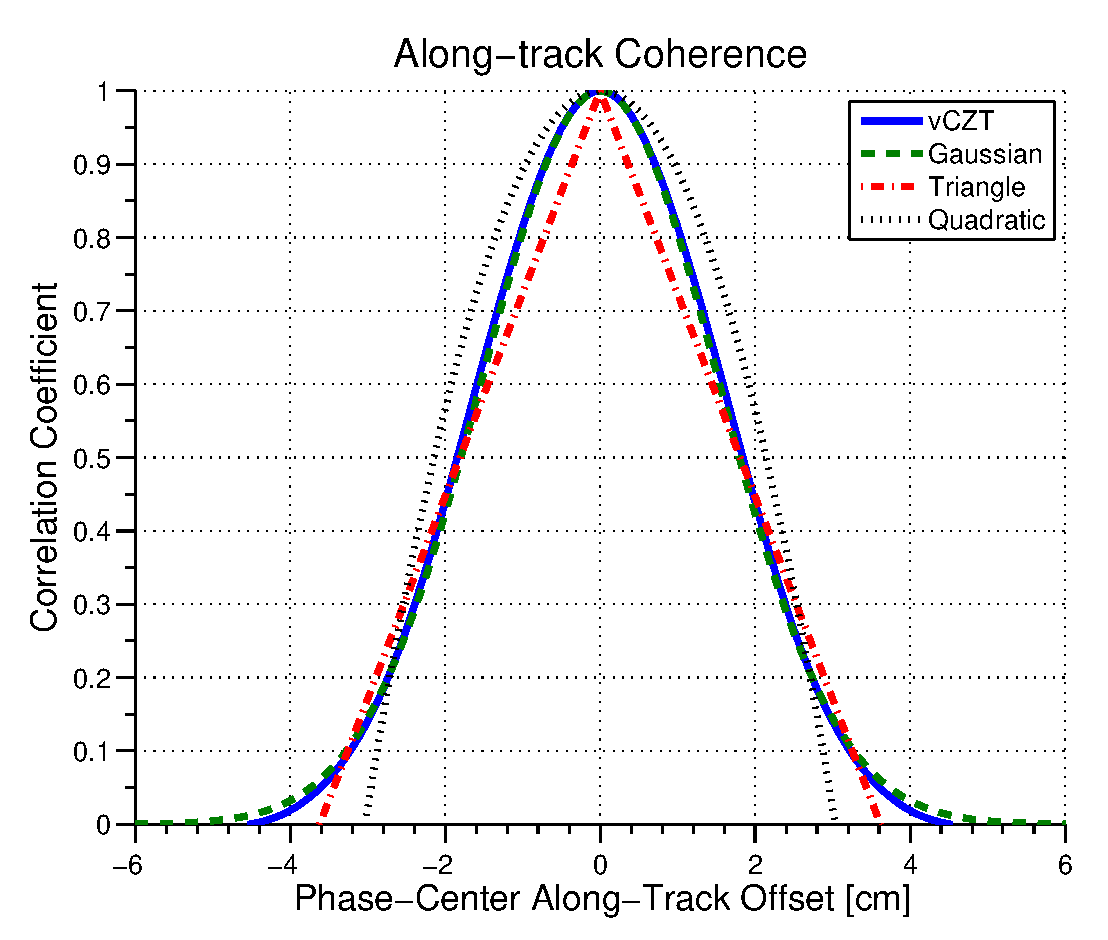
\includegraphics[width=\columnwidth]{sasCoherence.eps}
    \caption{The along-track spatial coherence for a system with directional transmit and receive beams is best modeled using a Gaussian function}\label{fig:sasCoherence}
\end{figure}

\begin{figure}[t]
    \centering
    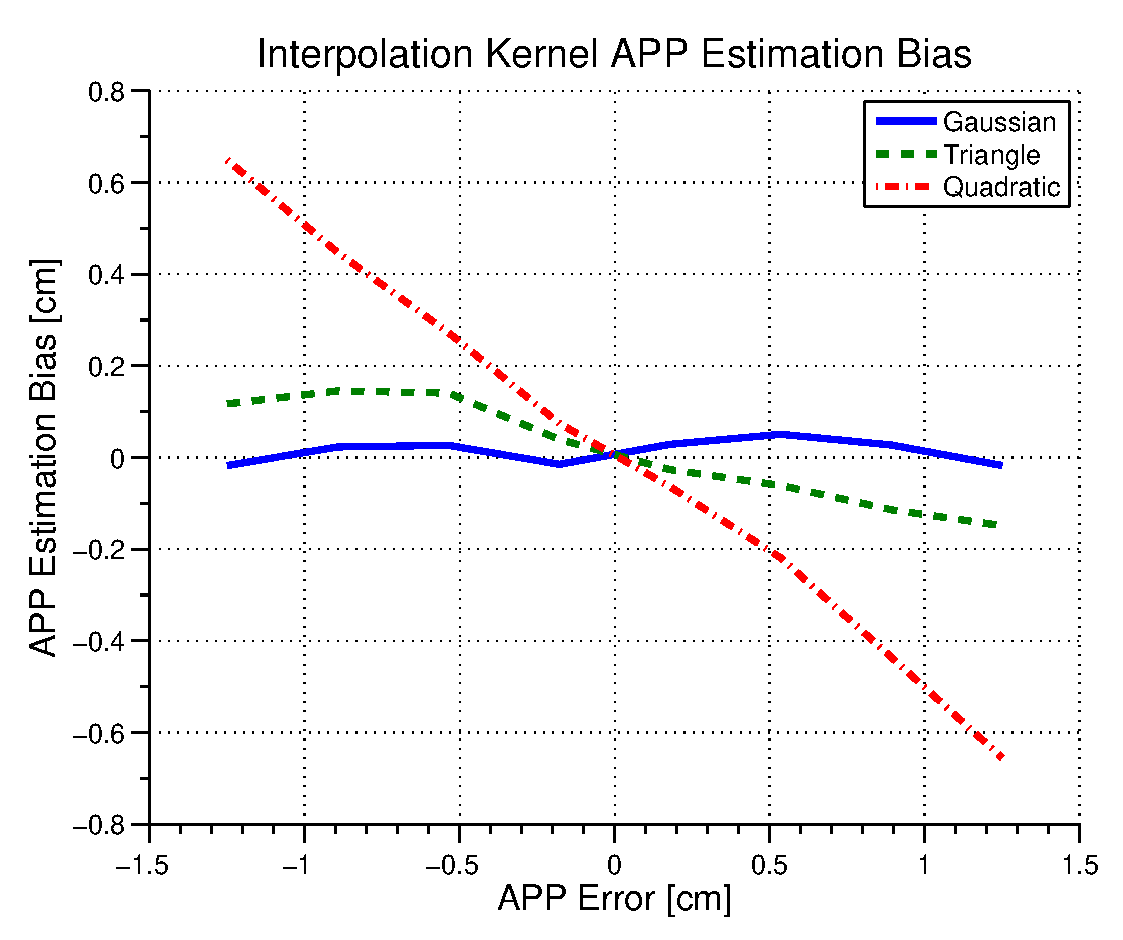
\includegraphics[width=\columnwidth]{dpcBias.eps}
    \caption{APP estimation bias errors are minimized by matching the interpolation kernel to the spatial coherence}\label{fig:dpcBias}
\end{figure}

\section{Comparison of Image Quality with Quadratic and Gaussian Interpolation Kernels}
The interpolation kernels shown in the prior section have been applied to the problem of along-track motion estimation for a pair of SAS data sets. The first data set was collected near Boston, Massachusetts. This data set was typical and the imagery did not exhibit any significant signs of defocusing due to along-track motion errors. The second data set was collected near Panama City, Florida. This data set was atypical and it exhibited significant defocusing due to along-track motion errors that were induced by an error in the navigation system for a portion of the collection. Each of these data sets were beamformed three times with three different methods of along-track motion estimation. The imagery was formed using the motion solution calculated by the built-in Inertial Navigation Sensor (INS). This approach assumes the sensors own along-track motion estimate is sufficient for producing high-quality imagery. The imagery is then generated using the quadratic and Gaussian interpolation kernels discussed above.

An example of the focus quality improvement of the Gaussian estimator over the INS estimator is shown in Figure~\ref{fig:imageComp}. This data is selected from the Panama City trial set. In Figure~\ref{fig:appIns}, the INS estimator is used and the resulting image shows significant along-track defocus. Using the Gaussian estimator and re-beamforming this data produces Figure~\ref{fig:appGaussian}.
%
\begin{figure*}[ht]
  \centering
  \hfill
  % Requires \usepackage{graphicx}
  \subfloat[INS APP Estimation]{\label{fig:appIns}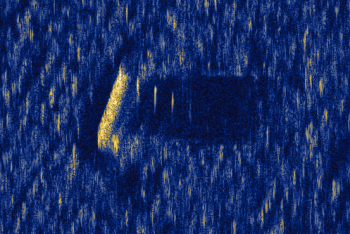
\includegraphics[width=\columnwidth]{appIns.png}}
  \hfill
  \subfloat[Gaussian APP Estimation]{\label{fig:appGaussian}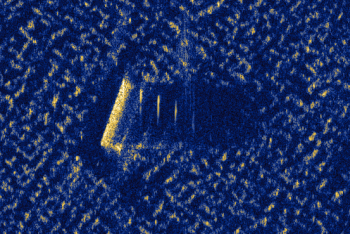
\includegraphics[width=\columnwidth]{appGaussian.png}}
  \hfill
  \caption{Significant APP error produces a very poorly focused image. Applying the Gaussian APP estimator significantly improves the image. This change in quality represents a $\Delta Q \approx 600$.} \label{fig:imageComp}
\end{figure*}

Figure~\ref{fig:imageComp} qualitatively shows a significant improvement in image quality for this specific image. To broadly assess the performance of the proposed interpolation kernels, a quantitative measure of image quality is needed. The metric must be able to quantify the change in image quality achieved by application of the along-track estimator. A well formed SAS image will have highly focused highlights and deep shadows. Image contrast can then be used as a measure of image quality; however, it is not an absolute measure of the quality since the contrast is partially dependent on the scene content. For a given set of data, the change in image contrast would provide a relative measure of quality that is less dependent on the scene content. The change in the contrast between two images formed with and without along-track motion estimation provides a measure of relative image quality quantifying the performance of each interpolation kernel.

A number of measures for image contrast exist \cite{Peters:1990a}. The contrast is defined here as a mean-normalized pixel variance
%
\begin{equation} \label{eq:imageQuality}
  Q = 1000\Bigl( \frac{\brkt{x^2}-\brkt{|x|}^2}{\brkt{|x|}^2} \Bigr),
\end{equation}
%
where $x$ is the pixel value and the ensemble $\brkt{\cdot}$ was taken over a \unit[2]{m} x \unit[2]{m} subset of the image. This metric is calculated across a non-overlapping grid over the full scene. For each image, the median of these measures was used to assign an overall quality to each image. Again, it is important to note that this is not an absolute measure of quality. In fact, $Q$, which is related to lacunarity, has been linked to the image complexity \cite{Williams:2015a}. Here, this metric is used as a measure of the relative quality when comparing two images made from the same data with different processing approaches. In this way, an increase in $Q$ between two different processing streams indicates improved image quality. A qualitative assessment of this metric for the scenes under test is a change of 20 points is the limit of observability, 100 points is noticeable, and 250 points or more is significant.

To assess quality, the data from a given test is beamformed with the INS measurement of the APP to form the baseline quality score. Next, the same data is beamformed with both the quadratic and Gaussian interpolators. The baseline quality score was subtracted from these two scores to produce an estimate of the relative image quality, $\Delta Q$.

Relative image quality scores have been calculated for the Boston and Panama City trials. Histograms of these scores are shown in Figure~\ref{fig:bostonPanamaCity}. As noted above, the Boston data showed no obvious visual APP errors, and the relative image quality scores reflect this Figure~\ref{fig:bostonHist}. Across the full data set, the two approaches resulted in mostly minor improvements to the scene contrast. This indicates there was some residual APP error; however, it is not substantially degrading the imagery. The histogram of scores for the Panama City data set indicates the presence of significant APP error, Figure~\ref{fig:pcbHist}. Many images show $\Delta Q > 100$ for both the quadratic and Gaussian kernels. Note that for both data sets the Gaussian kernel outperforms the quadratic as indicated by the heavier tailed relative quality distribution.

\begin{figure*}[!t]
  \centering

  % Requires \usepackage{graphicx}
  \subfloat[Boston Trial]{\label{fig:bostonHist}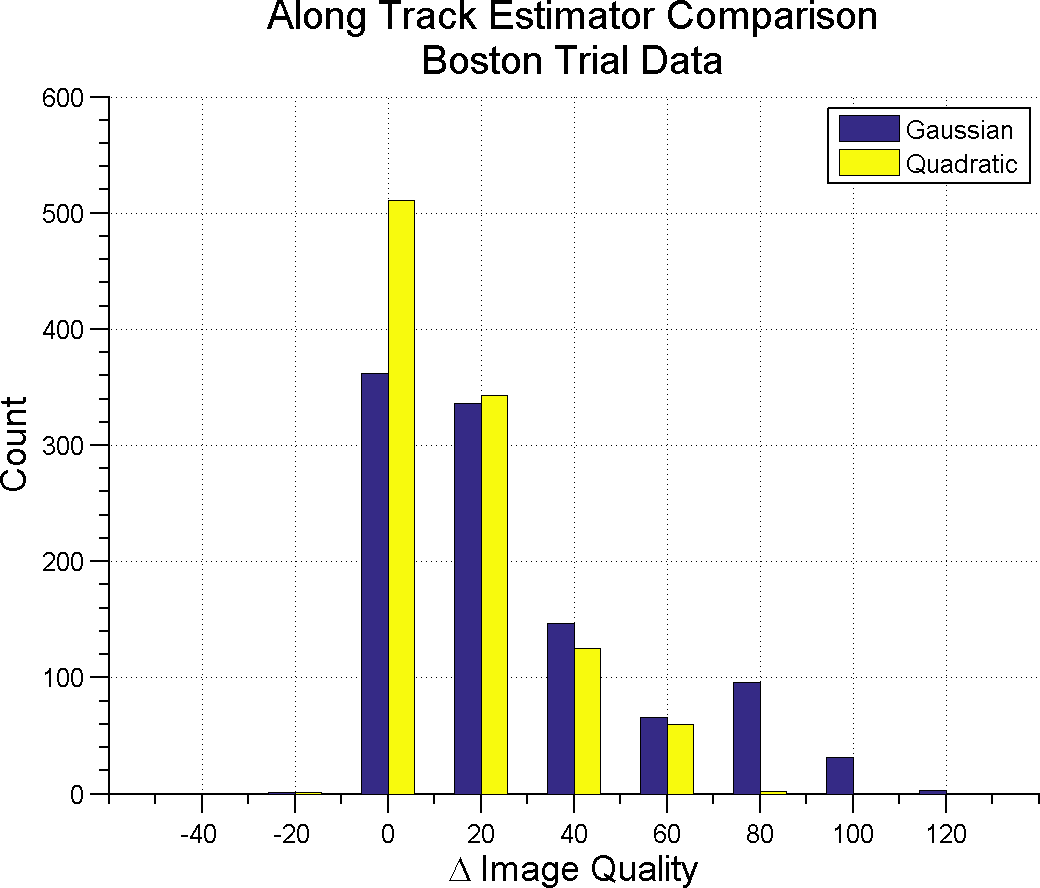
\includegraphics[width=\columnwidth]{input/bostonHistTrim.png}}
  \hfill
  \subfloat[Panama City Trial]{\label{fig:pcbHist}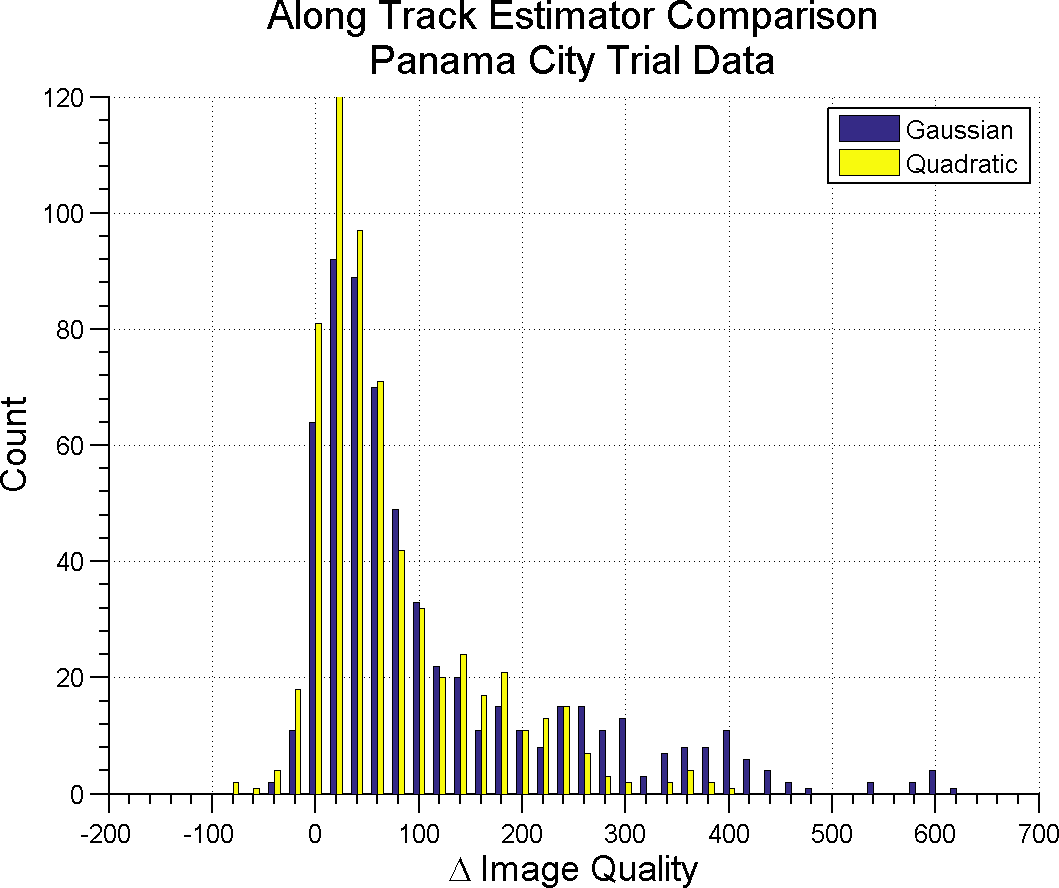
\includegraphics[width=\columnwidth]{input/pcbHistTrim.png}}

  \caption{The Gaussian interpolator provided a larger improvement in image quality in sea test conducted in Boston, MA and Panama City, FL.} \label{fig:bostonPanamaCity}
\end{figure*}



% An example of a floating figure using the graphicx package.
% Note that \label must occur AFTER (or within) \caption.
% For figures, \caption should occur after the \includegraphics.
% Note that IEEEtran v1.7 and later has special internal code that
% is designed to preserve the operation of \label within \caption
% even when the captionsoff option is in effect. However, because
% of issues like this, it may be the safest practice to put all your
% \label just after \caption rather than within \caption{}.
%
% Reminder: the "draftcls" or "draftclsnofoot", not "draft", class
% option should be used if it is desired that the figures are to be
% displayed while in draft mode.
%
%\begin{figure}[!t]
%\centering
%\includegraphics[width=2.5in]{myfigure}
% where an .eps filename suffix will be assumed under latex,
% and a .pdf suffix will be assumed for pdflatex; or what has been declared
% via \DeclareGraphicsExtensions.
%\caption{Simulation results for the network.}
%\label{fig_sim}
%\end{figure}

% Note that the IEEE typically puts floats only at the top, even when this
% results in a large percentage of a column being occupied by floats.


% An example of a double column floating figure using two subfigures.
% (The subfig.sty package must be loaded for this to work.)
% The subfigure \label commands are set within each subfloat command,
% and the \label for the overall figure must come after \caption.
% \hfil is used as a separator to get equal spacing.
% Watch out that the combined width of all the subfigures on a
% line do not exceed the text width or a line break will occur.
%
%\begin{figure*}[!t]
%\centering
%\subfloat[Case I]{\includegraphics[width=2.5in]{box}%
%\label{fig_first_case}}
%\hfil
%\subfloat[Case II]{\includegraphics[width=2.5in]{box}%
%\label{fig_second_case}}
%\caption{Simulation results for the network.}
%\label{fig_sim}
%\end{figure*}
%
% Note that often IEEE papers with subfigures do not employ subfigure
% captions (using the optional argument to \subfloat[]), but instead will
% reference/describe all of them (a), (b), etc., within the main caption.
% Be aware that for subfig.sty to generate the (a), (b), etc., subfigure
% labels, the optional argument to \subfloat must be present. If a
% subcaption is not desired, just leave its contents blank,
% e.g., \subfloat[].


% An example of a floating table. Note that, for IEEE style tables, the
% \caption command should come BEFORE the table and, given that table
% captions serve much like titles, are usually capitalized except for words
% such as a, an, and, as, at, but, by, for, in, nor, of, on, or, the, to
% and up, which are usually not capitalized unless they are the first or
% last word of the caption. Table text will default to \footnotesize as
% the IEEE normally uses this smaller font for tables.
% The \label must come after \caption as always.
%
%\begin{table}[!t]
%% increase table row spacing, adjust to taste
%\renewcommand{\arraystretch}{1.3}
% if using array.sty, it might be a good idea to tweak the value of
% \extrarowheight as needed to properly center the text within the cells
%\caption{An Example of a Table}
%\label{table_example}
%\centering
%% Some packages, such as MDW tools, offer better commands for making tables
%% than the plain LaTeX2e tabular which is used here.
%\begin{tabular}{|c||c|}
%\hline
%One & Two\\
%\hline
%Three & Four\\
%\hline
%\end{tabular}
%\end{table}


% Note that the IEEE does not put floats in the very first column
% - or typically anywhere on the first page for that matter. Also,
% in-text middle ("here") positioning is typically not used, but it
% is allowed and encouraged for Computer Society conferences (but
% not Computer Society journals). Most IEEE journals/conferences use
% top floats exclusively.
% Note that, LaTeX2e, unlike IEEE journals/conferences, places
% footnotes above bottom floats. This can be corrected via the
% \fnbelowfloat command of the stfloats package.




\section{Conclusion}
Synthetic aperture sonar image quality is negatively impacted by uncompensated errors in the along-track motion of the sensor. By making measurements of the along-track spatial coherence of the scattered field it is possible to create accurate estimates of the sensor's advance per ping. It was found that this type of estimation requires an accurate model for the spatial coherence of the scattered field. Application of the van Cittert-Zernike theorem to the problem of pulsed active sonar systems showed the spatial coherence for a typical high-frequency SAS collection geometry is well approximated by a Gaussian whose width is proportional to the sensor's element size.

Gaussian and quadratic along-track interpolation kernels were compared for a pair of at sea data collections. A relative image quality metric, based on image contrast, was defined to quantitatively assess the performance of the pair of interpolation kernels. In both tests, the use of an along track estimator was shown to provide improved image quality. Also in both tests, the performance of the Gaussian kernel exceeded the quadratic kernel.

% conference papers do not normally have an appendix


% use section* for acknowledgment
\section*{Acknowledgment}
The authors would like to acknowledge the US Office of Naval Research for their support of this research. The work shown here was conducted under ONR grants N00014-14-1-0566, N00014-16-1-2313.

Additionally, the authors would like to thank Steve Wagner for his implementation of the along-track interpolation kernels within the SAS image processing toolset.

\IEEEtriggeratref{12}

% trigger a \newpage just before the given reference
% number - used to balance the columns on the last page
% adjust value as needed - may need to be readjusted if
% the document is modified later
%\IEEEtriggeratref{8}
% The "triggered" command can be changed if desired:
%\IEEEtriggercmd{\enlargethispage{-5in}}

% references section

% can use a bibliography generated by BibTeX as a .bbl file
% BibTeX documentation can be easily obtained at:
% http://mirror.ctan.org/biblio/bibtex/contrib/doc/
% The IEEEtran BibTeX style support page is at:
% http://www.michaelshell.org/tex/ieeetran/bibtex/
\bibliographystyle{./bib/IEEEtran}
% argument is your BibTeX string definitions and bibliography database(s)
\bibliography{./bib/IEEEabrv,./bib/dcbPaperDatabase}
%
% <OR> manually copy in the resultant .bbl file
% set second argument of \begin to the number of references
% (used to reserve space for the reference number labels box)
%\begin{thebibliography}{1}
%
%\bibitem{IEEEhowto:kopka}
%H.~Kopka and P.~W. Daly, \emph{A Guide to \LaTeX}, 3rd~ed.\hskip 1em plus
%  0.5em minus 0.4em\relax Harlow, England: Addison-Wesley, 1999.
%
%\end{thebibliography}




% that's all folks
\end{document}


